\chapter{Framework}
\label{chapter:framework}

This chapter explains the main \textit{building blocks} for \textbf{problem dimensionality reduction}, \textbf{database generation}, and \textbf{machine learning setup}. It will underscore the \textit{key role} of \textbf{parametrization} in the \textbf{dimensionality reduction} of the database, in terms of its \textbf{dimensions} and the way of \textbf{representing} the data.

\section{Blade Geometry Parametrization}

The blade geometry is defined by two components: the \textbf{camberline} and the \textbf{profile line}. The following parametrization follows \textbf{Kulfan's parametrization} \cite{kulfan2008universal}.

\subsection{Camberline}

The camberline serves as a \textit{primary property layer} for defining the blade geometry. The suction side and pressure side geometry are added atop this \textit{layer} to generate the complete blade. The \textbf{camberline} holds the utmost importance in blade generation. Even a \textit{minor} alteration to the camberline shape can lead to a \textit{significant} change in the flow behavior around the blade.

\subsubsection{Formulation}

The parameters used for camberline definition are:

\begin{itemize}
  \item $\gamma$: stagger angle.
  \item $\chi_1$: metal inlet angle.
  \item $\chi_2$: metal outlet angle.
\end{itemize}

These three parameters ($\gamma$, $\chi_1$, and $\chi_2$) are then employed to compute \textit{intermediate variables}, which will subsequently contribute to defining the camberline structure. The \textit{intermediate variables} $n$, $a$, and $b$ are computed as:

\begin{align}
  n & = \frac{tan(\chi_2) + tan(\chi_1)}{tan(\gamma)} \\
  a & = \frac{tan(\chi_2)}{n} \\
  b & = - \frac{tan(\chi_1)}{n}
\end{align}

The camberline is defined as:

\begin{align}
  y          & = a \cdot x^n + b \cdot (1 - x)^n \\
  y^{\prime} & = a \cdot n \cdot x^{n-1} - b \cdot n \cdot (1 - x)^{n - 1} \\
  \boldsymbol{n} & = 
  \begin{bmatrix}
    n_x \\
    n_y
  \end{bmatrix} =
  \begin{bmatrix}
    - \frac{y^{\prime}}{\sqrt{1 + (y^{\prime})^2}} \\
    \frac{1}{\sqrt{1 + (y^{\prime})^2}}
  \end{bmatrix}
\end{align}

Figures~\ref{fig:cLine1} and~\ref{fig:cLine2} depict two potential camberlines.

\begin{figure}[!h]
  \centering
  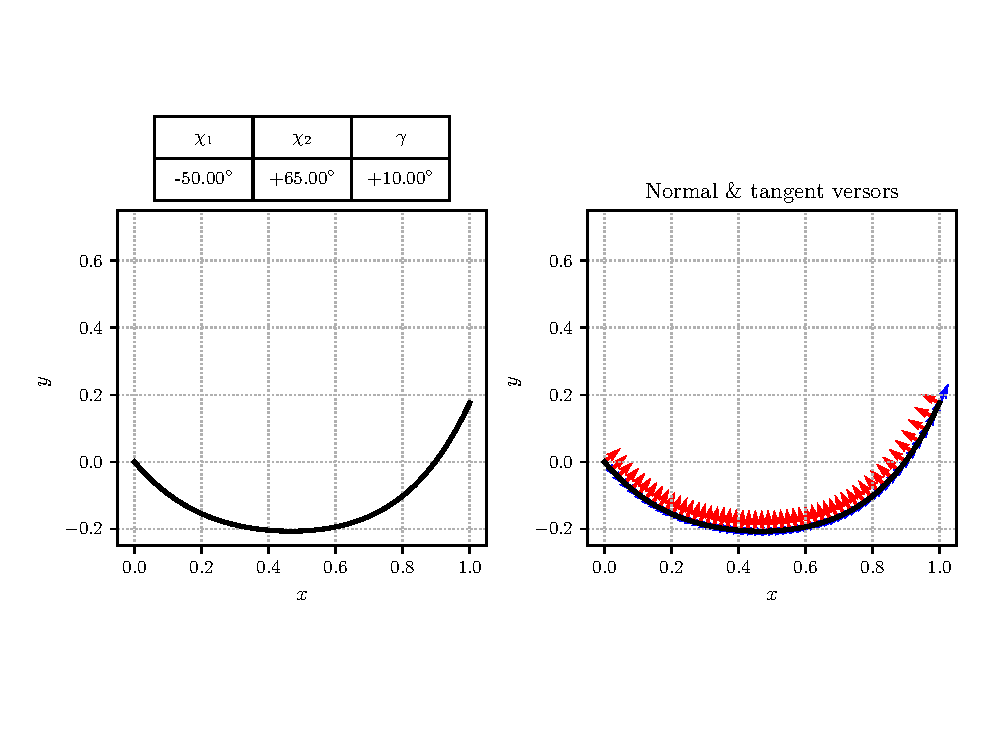
\includegraphics[width=1\linewidth, trim=0cm 1.5cm 0cm 1cm, clip]{pyFigure/figures/cLine1.eps}
  \caption{Camberline: $\gamma = 10^{\circ}$, $\chi_1 = -50^{\circ}$, and $\chi_2 = 65^{\circ}$.}
  \label{fig:cLine1}
\end{figure}

\begin{figure}[!h]
  \centering
  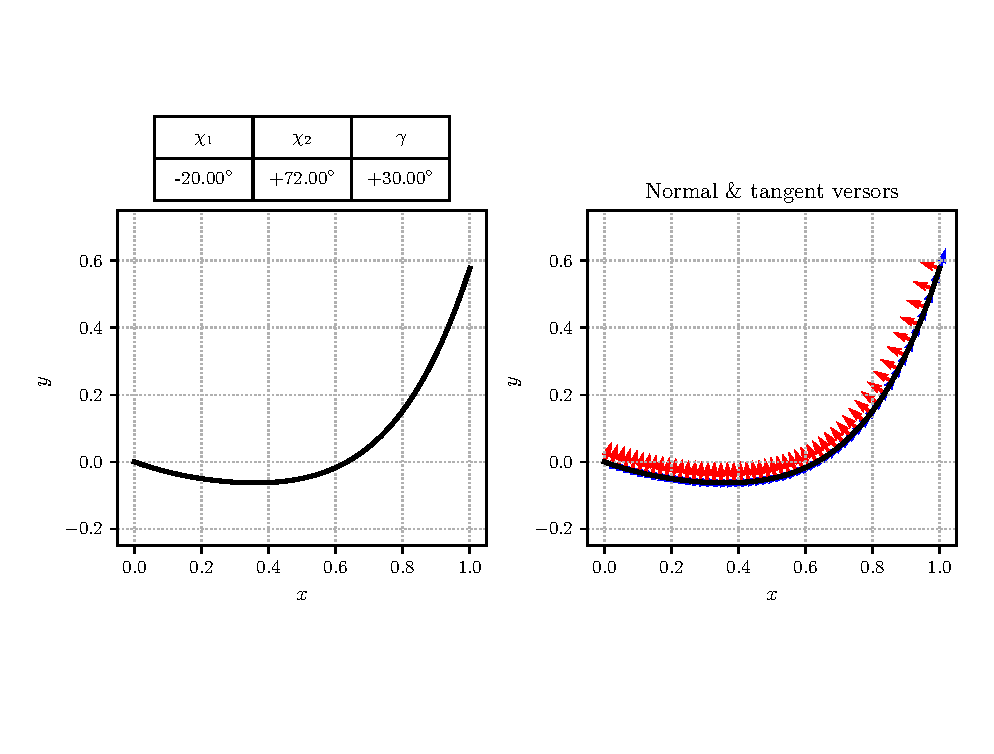
\includegraphics[width=1\linewidth, trim=0cm 1.5cm 0cm 1cm, clip]{pyFigure/figures/cLine2.eps}
  \caption{Camberline: $\gamma = 30^{\circ}$, $\chi_1 = -20^{\circ}$, and $\chi_2 = 70^{\circ}$.}
  \label{fig:cLine2}
\end{figure}

The normal and tangent vectors are employed for the thickness distribution along the camberline, as explained in Section~\ref{sec:profileLine}.

\subsection{Profile Line}
\label{sec:profileLine}

The profile line defines both the \textbf{suction side} and the \textbf{pressure side} of the blade. Utilizing \textbf{Kulfan's parametrization} \cite{kulfan2008universal}, it is possible to generate a wide array of blades \textbf{using just a few parameters}. The preference for parametrization over coordinate-based representation arises from:

\begin{itemize} 
  \item optimization \textbf{speed} 
  \item the fact that, considering the tool's ultimate purpose, parameters are \textbf{easier to correlate} than a pure coordinate-based representation
\end{itemize}

\subsubsection{Formulation}

The profile line is defined by $N + 1$ parameters: $A_i \text{ for } i = 0:N$. These parameters represent the \textbf{weights} of the \textbf{modes} that characterize the blade.

\paragraph{Bernstein Functions}

The shape modes of the blade are described by the Bernstein functions, denoted as $S_{(x, i, N)}$:

\begin{equation}
  S_{(x, i, N)} = A_i \cdot \frac{N!}{(N - i)! \cdot i!} \cdot x^i \cdot (1 - x)^{N - 1} \text{, for } i = 0:N
  \label{eqn:bernstein}
\end{equation}

The blade geometry modes are visualized in Figure~\ref{fig:bernstein}.

\begin{figure}[!h]
  \centering
  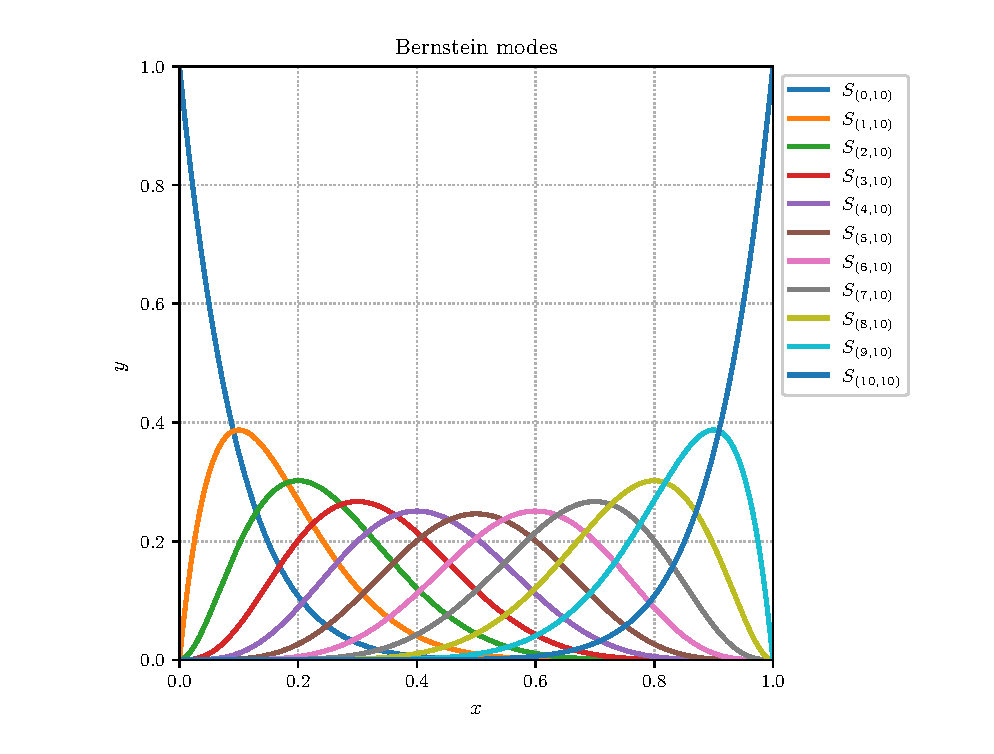
\includegraphics[scale=1]{pyFigure/figures/bernstein.eps}
  \caption{Bernstein function, $S_{(x, i, N)}$, with $A_i = 1$ and $N = 10$.}
  \label{fig:bernstein}
\end{figure}

\paragraph{Shape Function}

In addition to the Bernstein functions as described in Equation~(\ref{eqn:bernstein}), a \textbf{shape function}~\cite{kulfan2010recent} is introduced for representing the \textit{leading edge properties} and \textit{trailing edge properties} of the blade. The shape function, denoted as $C_{(x)}$, takes the form:

\begin{equation}
  C_{(x)} = x^{C_0} \cdot (1 - x)^{C_1}, \text{ where: } C_0 = 0.5 \text{ and } C_1 = 1.0
  \label{eqn:shapeFunction}
\end{equation}

Equation~(\ref{eqn:shapeFunction}) captures the \textit{roundness} of the leading edge and the wedge angle properties at the trailing edge of the blade. The shape function is illustrated in Figure~\ref{fig:shapeFunction}.

\begin{figure}[!h]
  \centering
  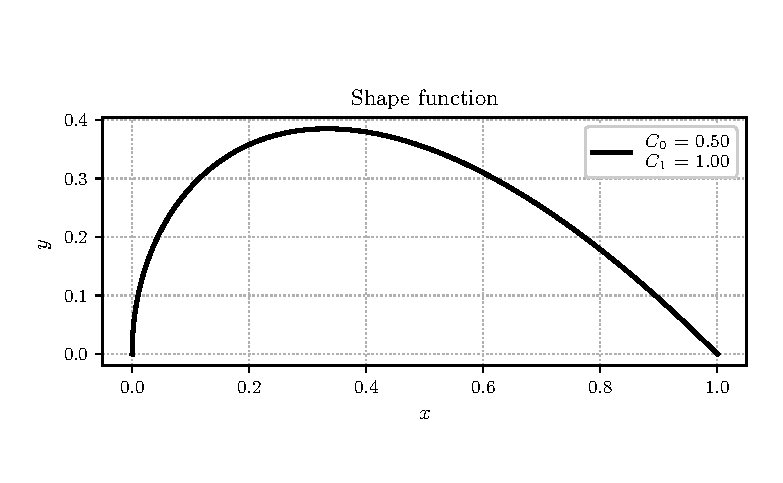
\includegraphics[scale=0.8]{pyFigure/figures/class.eps}
  \caption{Shape function, $C_{(x)}$.}
  \label{fig:shapeFunction}
\end{figure}

\paragraph{Thickness Distribution}

The blade thickness, denoted as $\zeta$, is determined by combining Equation~(\ref{eqn:bernstein}) and Equation~(\ref{eqn:shapeFunction}). Additionally, the trailing edge radius, $R_{TE}$, is incorporated using a linear distribution, $\zeta_{TE}$, over the camberline. The thickness distribution $\zeta_{(x)}$ is related to camberline properties and \textbf{is distributed using a unit Bernstein function} - $S_{(x, 0, 2)}$. The distribution $\zeta_{TE_{(x)}}$ solely relies on camberline properties $n_x$ and $n_y$.

\begin{align}
  \zeta_{(x)}       & = \sum_{i = 0}^N S_{(x, i, N)} \cdot C_{(x)} \\
  \zeta_{TE_{(x)}}  & = x \cdot R_{TE} 
\end{align}

The pressure(suction) side ($\pm$) profile line coordinates are then computed as: 

\begin{align}
  x_{PS/SS} & = x_{camberline} \pm n_x \cdot \zeta_{(x)} \cdot S_{(x, 0, 2)} \pm n_x \cdot \zeta_{TE_{(x)}}\\ 
  y_{PS/SS} & = y_{camberline} \pm n_y \cdot \zeta_{(x)} \cdot S_{(x, 0, 2)} \pm n_y \cdot \zeta_{TE_{(x)}}+ \zeta_{(x)} \cdot \big[1 - S_{(x, 0, 2)}\big]
\end{align}

\begin{figure}[H]
    \centering
    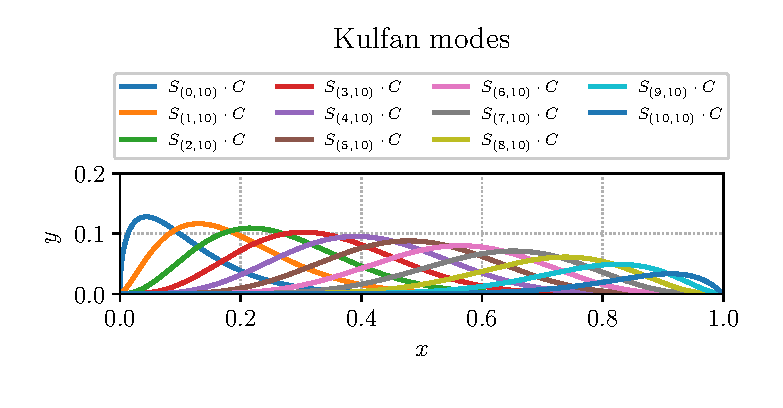
\includegraphics[scale=0.9]{pyFigure/figures/kulfan.eps}
    \caption{Kulfan modes, $S_{(x, i, N)} \cdot C_{(x)}$, with $A_i = 1$ and $N = 10$.}
    \label{fig:kulfan}
\end{figure}

Figures~\ref{fig:kulfan} presents the \textbf{profile blade modes}, which are a combination of Equation~(\ref{eqn:bernstein}) and Equation~(\ref{eqn:shapeFunction}).

The suction side and pressure side coordinates are computed using a \textit{custom set of points} over the camberline.
The camberline is discretized with \textbf{Chebyshev nodes} all along the chord. This approximation allows better accuracy at the leading edge and at the traling edge of the blade.

Figure~\ref{fig:bladeNodes} and Figure~\ref{fig:bladeNodes1} show clearly the blade coordinates starting from the chord discretization passing through the camberline discretization to the suction side and pressure side points.
Using the \textbf{Chebyshev nodes} allows having a \textbf{faster generation} of the blade while keeping \textbf{good accuracy} over the blade coordinates representation. 

\begin{figure}[H]
  \centering
  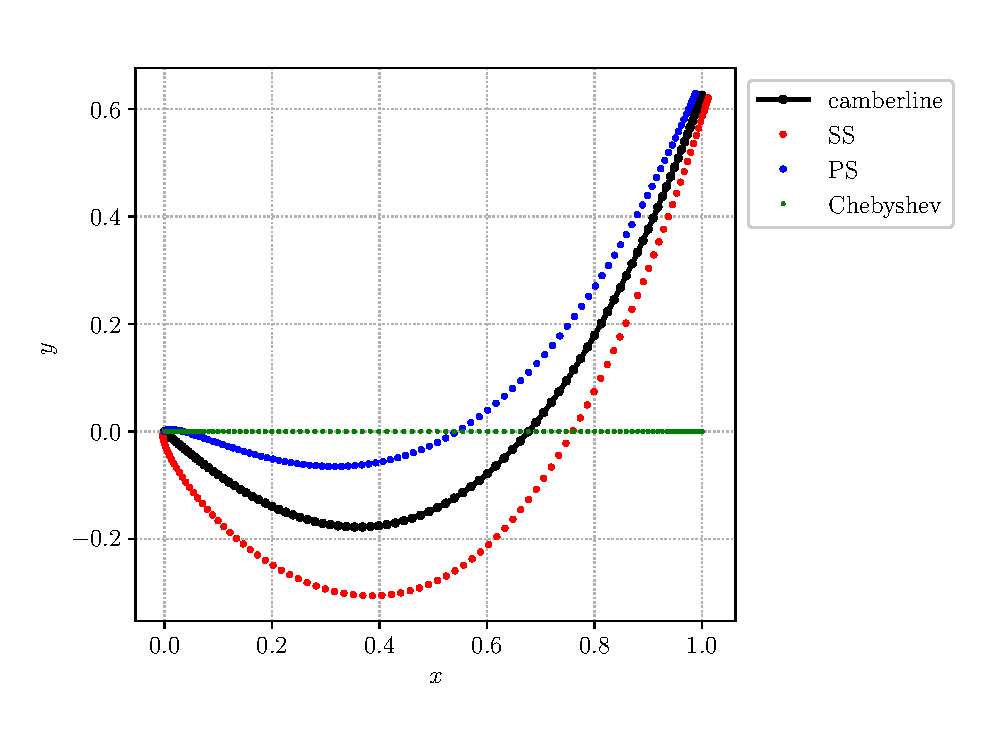
\includegraphics[scale=0.5]{pyFigure/figures/coordinate1.eps}
  \caption{Coordinate based representation of the blade.}
  \label{fig:bladeNodes}
\end{figure}

\begin{figure}[H]
  \centering
  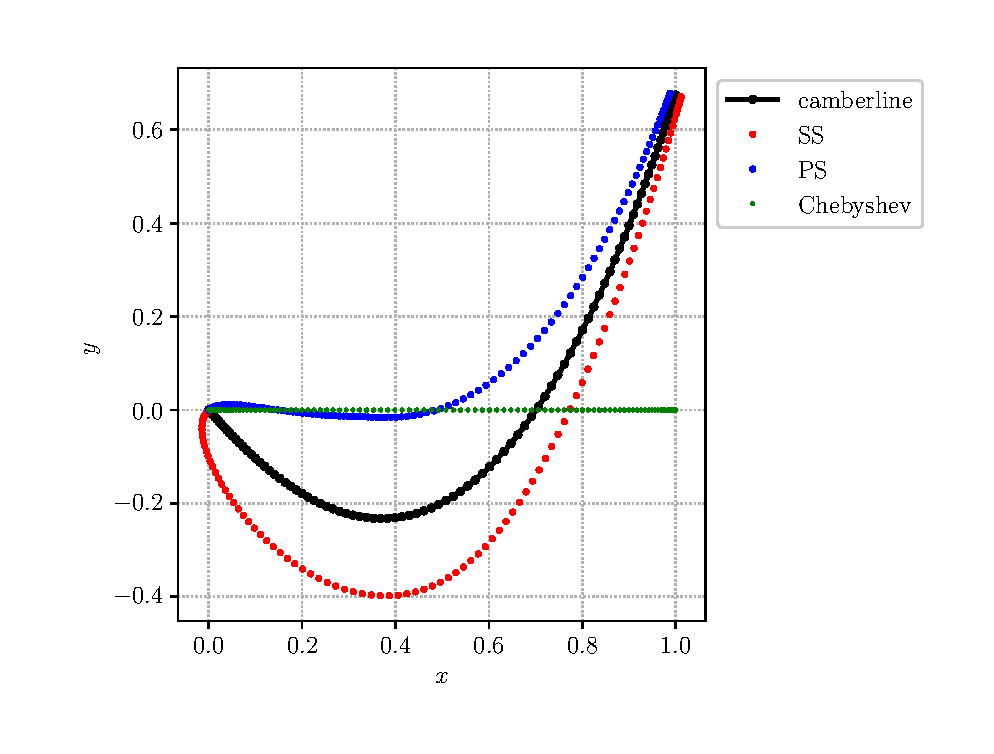
\includegraphics[scale=0.5]{pyFigure/figures/coordinate2.eps}
  \caption{Coordinate based representation of the blade.}
  \label{fig:bladeNodes1}
\end{figure}

\subsubsection{Main Features}

Kulfan's parametrization retains several crucial geometric properties:

\begin{itemize}
  \item The leading edge radius, $R_{LE}$, is determined solely by the $A_0$ parameter \cite[App. B]{kulfan2008universal}. $A_0 = \sqrt{2 \cdot R_{LE}}$.
  \item The trailing edge angle, $\beta$, is directly related to the $A_{N}$ parameter \cite[App. A]{kulfan2008universal}. $A_N = tan(\beta) + R_{TE}$.
\end{itemize}

These features hold great \textbf{significance} in studying the \textbf{blade characteristics} in relation to flow properties.

\subsubsection{Scaling}

The blade optimization takes place through \textbf{incremental steps}, utilizing a strategy that ensures \textit{faster convergence}. One key aspect of this strategy is to perform a \textbf{scaling} of the blade once convergence is achieved. 
This step is crucial for optimizing a blade with many degrees of freedom. 
The primary aim of scaling is to address potential \textit{pits} within the domain during the blade optimization.

This scaling is generated solving a linear system. The linear system uses a matrix of $N_{new} \ \times \ N_{new}$ dimension. 
To build up this matrix, the blade, parametrized with lower number of parameters $N$, is evaluated on an equispaced number of points, $N_{new}$ times, along the axial chord.  
The resulting matrix is then used to compute the new parametrization, made by $N_{new}$ parameters.

It's important to note that the only unaltered parameters are:

\begin{itemize}
    \item For the suction side and pressure side: $R_{LE}$ and $\beta$
    % \item For the pressure side: $R_{LE}$ and $\beta$
    \item For the camberline: $\chi_1$, $\chi_2$ and $\gamma$
    % \item $A_0$ \& $A_i$ for the suction side and the pressure side 
    % \item $A_0$ 
    % \item $A_i$ 
    % \item $\chi_1$
    % \item $\chi_2$
\end{itemize}

These parameters remain unchanged during the scaling process due to their direct correlation with the blade's geometrical properties

Figures~\ref{fig:blade01} and~\ref{fig:blade03} illustrate different blades and the outcomes resulting from their scaling.

\begin{figure}[H]
  \centering
  \hspace*{-3cm}
  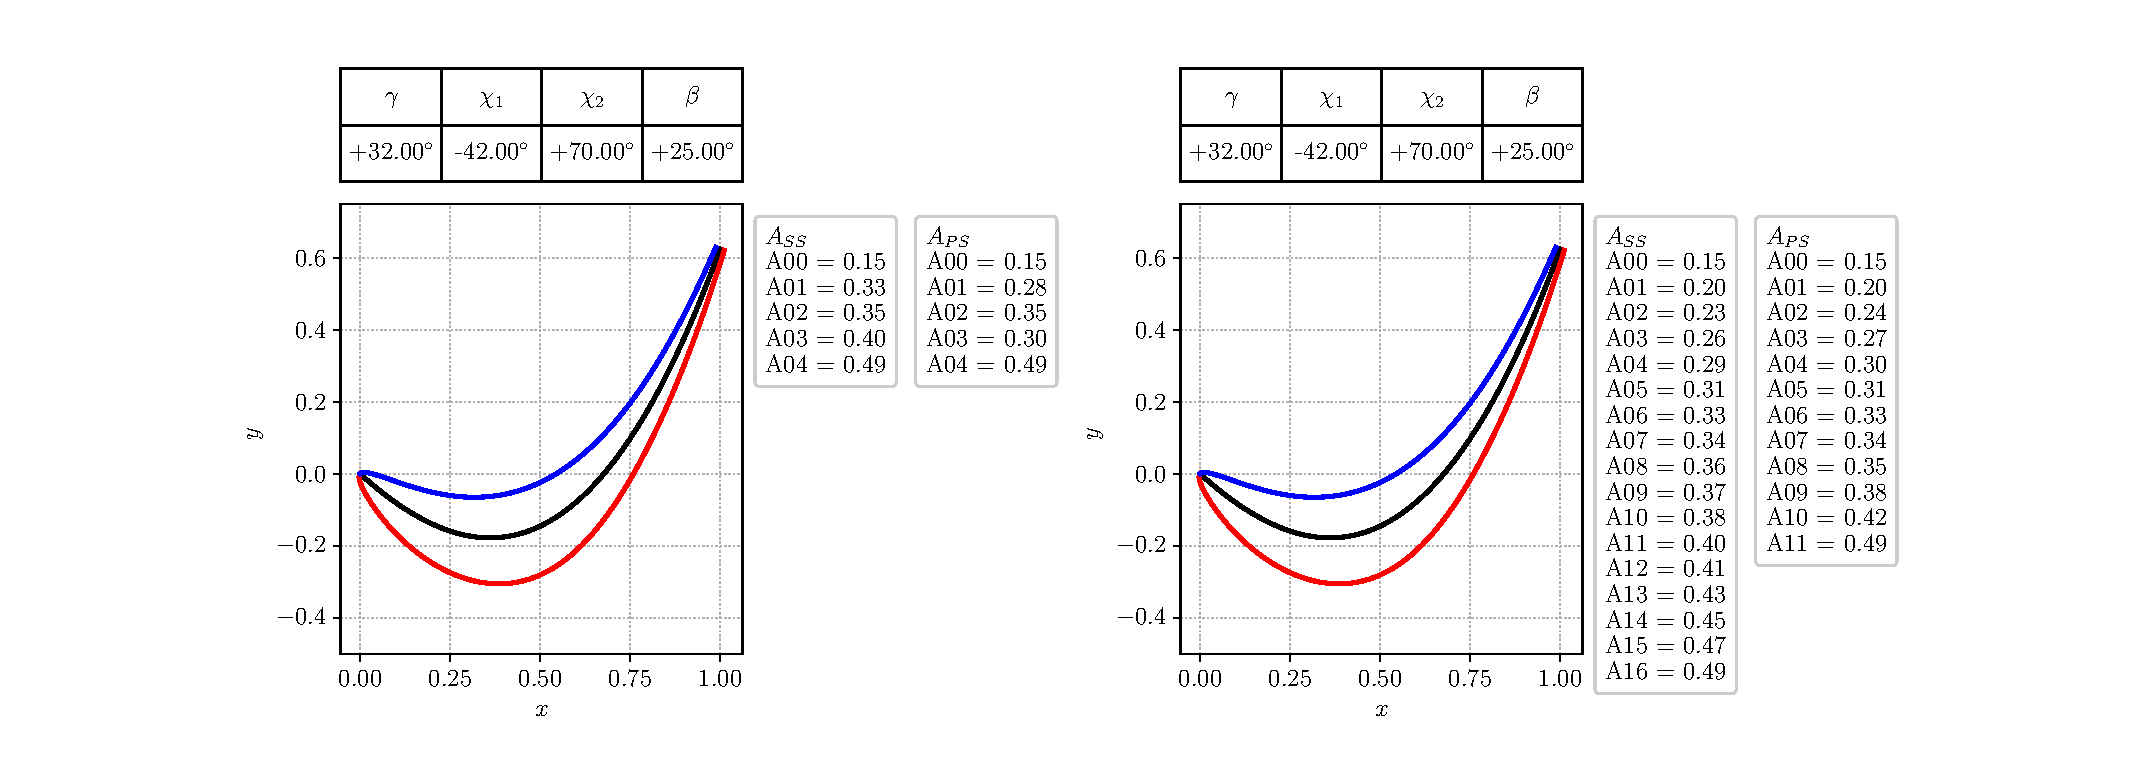
\includegraphics[width=1.35\textwidth]{pyFigure/figures/blade1.eps}
  \caption{Example No. 1 of blade scaling following Kulfan's parametrization.}
  \label{fig:blade01}
\end{figure}

\begin{figure}[H]
  \centering
  \hspace*{-3cm}
  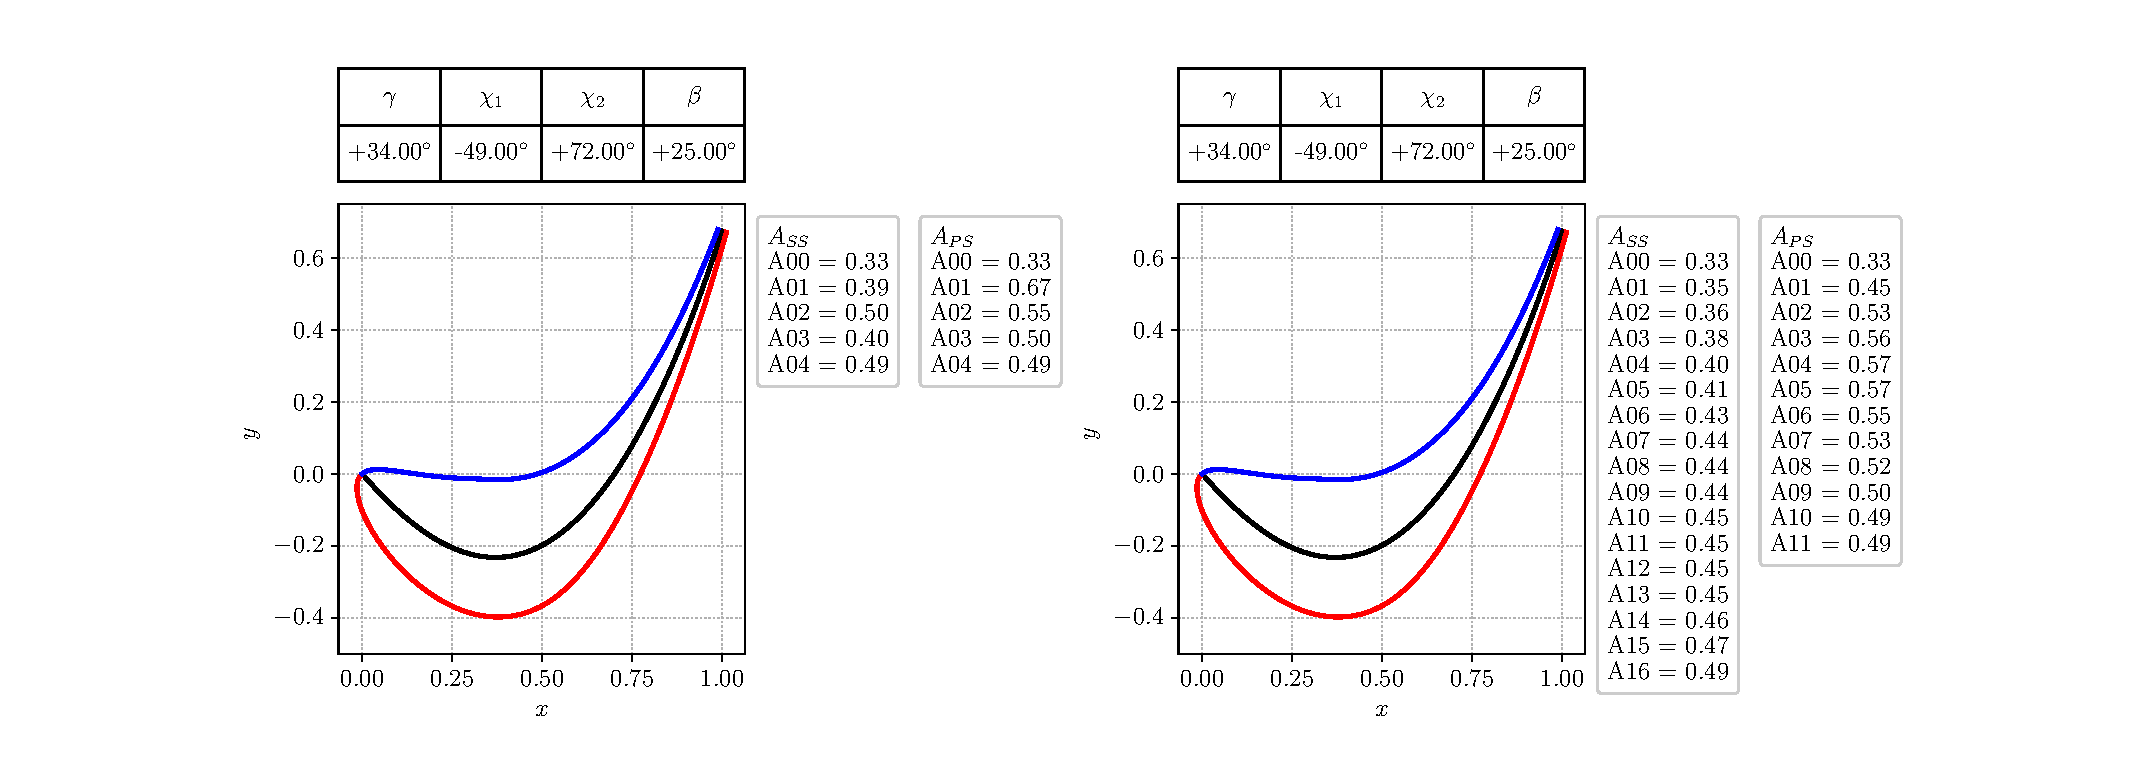
\includegraphics[width=1.35\textwidth]{pyFigure/figures/blade2.eps}
  \caption{Example No. 2 of blade scaling following Kulfan's parametrization.}
  \label{fig:blade03}
\end{figure}

\section{Aerodynamic Style Parametrization}
\label{sec:aeroStyle}

In contrast to the \textbf{aerodynamic duty}, the \textbf{aerodynamic style} allows to define locally the load distribution along the blade. 

The \textbf{aerodynamic style} is defined by the Mach fraction, $\frac{M}{M_{TE}}$, over the surface length fraction, $\frac{S}{S_{TOT}}$. 

There are multiple \textit{reasons} about the use of these parameters. The key ones are:

\begin{itemize}
  \item The leading edge is a regione where, due to the high curvature of the geometry, there is a \textbf{high change in surface fraction over the axial chord}. Since this region is a very important for the correlation study, the $\frac{M}{M_{TE}} \ vs \ \frac{S}{S_{TOT}}$ formulation results appropriate.
  \item The \textbf{boundary layer} properties, such as transition and detachament, is mostly dependent on the \textbf{total flow path length} done by the flow - described by $S$ - and not over its projection over the axis - described by $x$.
\end{itemize}

The \textbf{aerodynamic style}~\cite{clark2019step} is defined by these variables:

\begin{itemize}
  \item $\frac{M_{LE}}{M_{TE}} \frac{M_2}{M_1}$: leading edge Mach fraction. This parameter defines the load at the leading edge on the suction side.
  \item $\frac{M_{PEAK}}{M_{TE}}$: peak Mach fraction. Defines the peak Mach fraction on the suction side, representing the highest Mach value over the blade.
  \item $\frac{M_{PRESS}}{M_{TE}} \frac{M_2}{M_{1, ax}}$: pressure Mach number. It is a \textbf{double descriptor} of the leading edge load on the suction side and the Mach fraction before the Mach fraction raises to reach the trailing edge on the pressure side. 
  \item $\frac{S_{PEAK}}{S_{TOT}}$: surface fraction position where the peak Mach fraction, $\frac{M_{PEAK}}{M_{TE}}$, is positioned over the load distribution.
\end{itemize}

It is important to understand that \textbf{the load varies with respect to $\frac{M_1}{M_2}$ and $\frac{M_{1, ax}}{M_2}$}. This
is due to the fact that the leading edge load distribution is highly sensitive to the inlet flow properties\footnote{Defined by $M_1$ and $\alpha_1$.}. 

\subsection{Trial \& Error}

Having introduced the variables which define the loading distribution, it is important to notice that these variables have to 
be tuned in order to meet the manufacturing requirements - such as the leading edge radius ($\frac{R_{LE}}{c} \geq 1.25 \cdot 10^{-2}$).
The trailing edge radius ($\frac{R_{TE}}{c}$) is set at $1.25 \cdot 10^{-2}$ throughout the whole study. These values are dictated mainly by the manufacturing capabilities in the turbomachinery industry. 

This concept is very important because there are blades which might not satisfy both the aerodynamic style and the duty imposed.
The trial and error tuning of the loading behavior at the leading edge can be seen as a design limit but it can be also seen as a first \textit{filtering operation} 
over the aerodynamic style and the aerodynamic duty for appreciable results.

The \textbf{\textit{trial and error}} approach has been used mainly over the loading behavioiur at the leading edge 
- both at the suction side and the pressure side of the blade. These corrections are mainly made on the behavior of the 
conjunction point between the ellipse shaped loading at the leading edge with the straight line after it. 

This behavior is of paramount importance as it enables the convergence of a specific blade
set in terms of loading distribution and the exit flow angle.

Figures~\ref{fig:aerodynamicStyle} provide visualizations of the load properties obtained using a \textbf{spline parametrization}:

\begin{figure}[H]
  \centering
  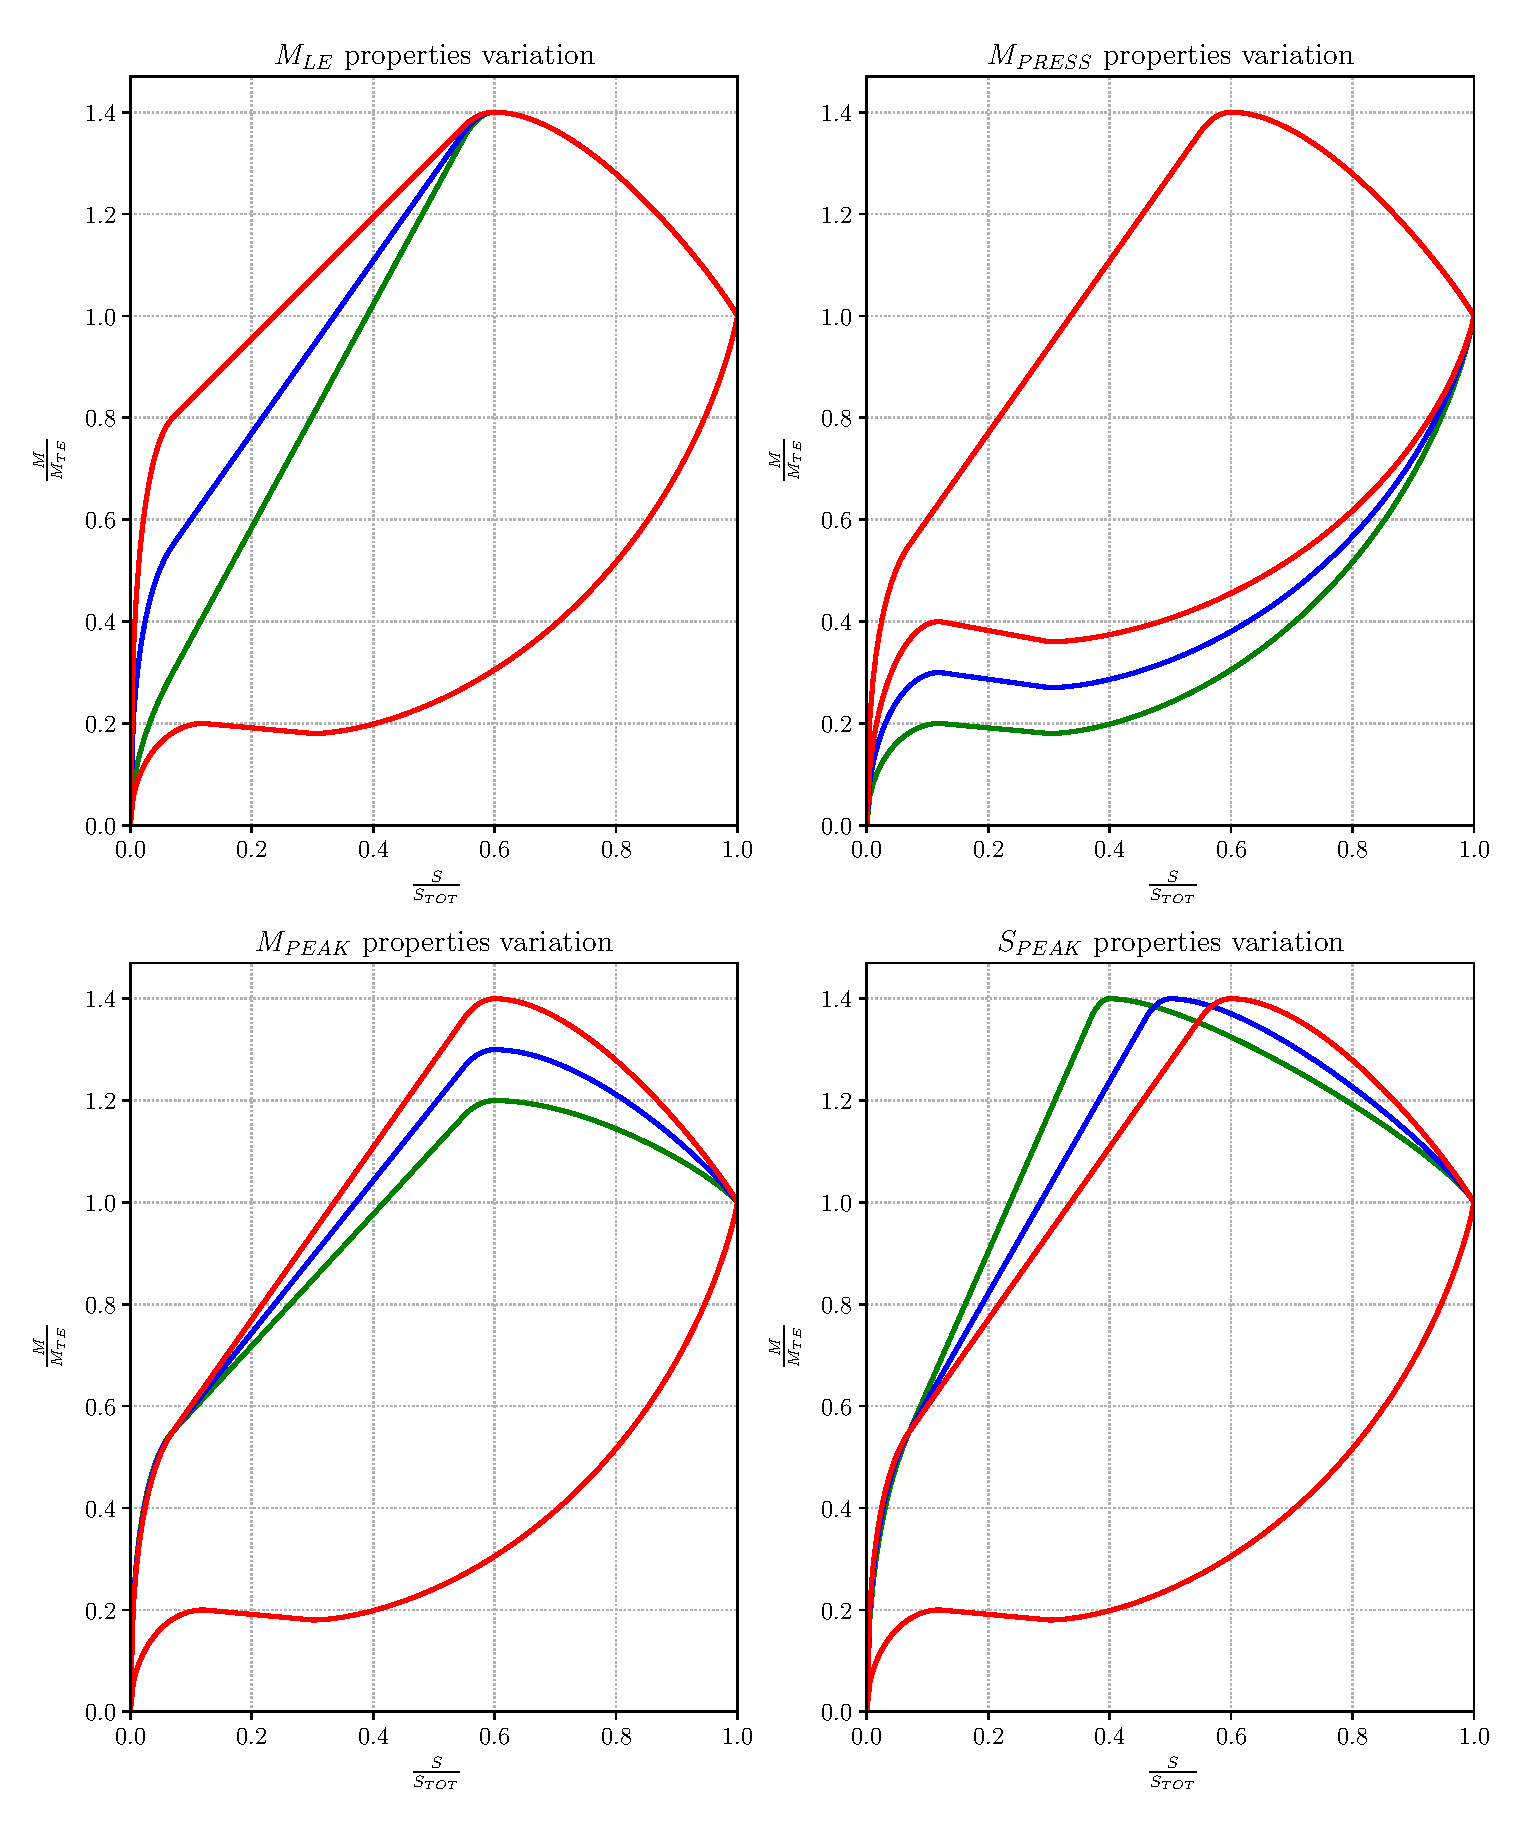
\includegraphics[scale=0.5]{pyFigure/figures/loadProperties.eps}
  \caption{Aerodynamic style properties.}
  \label{fig:aerodynamicStyle}
\end{figure}
